\chapter{Equalization}
\setheader{Equalization}
\label{chap:equalization}

In this chapter two things will be discussed.
At first a few adjustments are discussed to treat the recorded signals in such a way that they give the right results and to make sure they are displayed in the same dB-scales so they are comparable to each other.
After that some equalizing-theory is discussed to solve the problem of the influence of the acoustic system on the measurements, presented in the last chapter.
Which we will conclude with the solution for this problem and again some preliminary results and a short recap.

\section{Processing the recordings}
\label{sec:eq-proc_rec}
There are a few differences between different recordings.
For a start, the phones do not start with recording at the same time as the signal is played through the loudspeaker.
To compensate for these different delays, the impulse responses are altered so the delay is 141 samples (equation \eqref{eq:samples}) for all measurements.

The audio signal from the loudspeaker travels through space before it is recorded by the smartphone microphone.
Every measured impulse response thus needs to only consist of a part of the signal travelling through space and a part affected by the microphone.
The number of samples it would take the sound from the loudspeaker to the smartphone microphone is computable from the facts that the distance between the loudspeaker and the smartphone microphone is 1 meter, and the speed of sound and the sampling frequency are known too,

\begin{equation}
\label{eq:samples}
\dfrac{\text{distance}}{v_\text{air}} \cdot f_{s} = \frac{1}{344} \cdot 48000 \Rightarrow \left\lceil \frac{1}{344} \cdot 48000 \right\rceil = 141\text{ samples}.
\end{equation}

Next to this, there needs to be a `point of reference' to compare the measurements with different settings with each other and to choose a setting for the dB-scale.
In the presented results (Section \ref{sec:results}), the equalized gain of the smartphone microphone (labelled with number 6) at a frequency of $f=200$ Hz at $\theta=0^\circ$ and $\phi=90^\circ$ is chosen as a reference point of 0 dB.
Measurements with other settings will be referenced to this reference point via the measurements with the microphone.
The preliminary results in this chapter (Section \ref{sec:eq-prelim}) are calibrated to this point, the results in the rest of this thesis are.

\section{Equalizer design}
% theorie zegt: kan niet! (papers)  \cite{karjalainen2007equalization}
% om dit te bevestigen toch zelf op onderzoek uitgegaan:
% toeplitz: neh
% RLS: neh
% theorie wint, (non-minimum phase, te veel non-linearities) wij doen wel de log-equalization \cite{Thomas2006}
% Dus beamformer twee dingen testen.
\label{sec:eq-design}
\begin{figure}[b!]
    \centering
    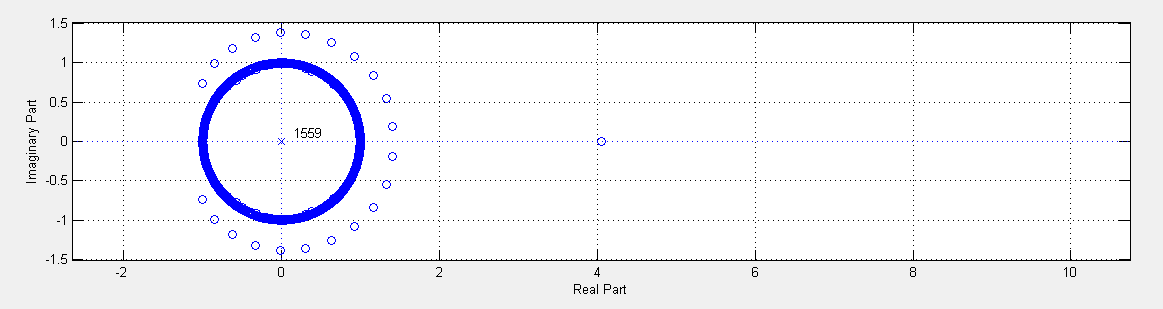
\includegraphics[width=\textwidth]{afbeeldingen/polezero.png}
    \caption[Pole-zero plot impulse response acoustic system]{The pole-zero plot for the 1559 first entries of the impulse response of the system, measured by the microphone \cite{manual:microphone}. This plot is generated by the \texttt{pdatool} in \matlab.}
    \label{fig:polezero}
\end{figure}
When measuring the impulse response of the microphone, also the impulse response of the acoustic system is taken into account (the acoustic system consists of: the loudspeaker, the audio interface (in this case the Fireface 800), the audio-amplifier and the cables).
To determine the impulse response of the microphone in the smartphone as good as possible, the impulse response of the acoustic system should be inverted.
Therefore the same measurements as with the smartphone are conducted with a microphone \cite{manual:microphone} with an almost perfect frequency response (Figure \ref{fig:app:hardware:mic}).

The response of a system can be written as \eqref{eqn:system} in the $z$-domain \cite[eq.~(5.4.6)]{book:dsp}. 
The zeros of the system are the zeros of $A(z)$ and the poles of the system are the zeros of $B(z)$,
\begin{equation}
\label{eqn:system}
H(z)=\dfrac{A(z)}{B(z)}.
\end{equation}

If a system is minimum phase \cite[p.~331-337]{book:dsp}, meaning it is causal and invertible, the inverse of the system is relatively easy to determine.
A minimum phase system is easy to recognise by its pole-zero plot.
If all poles and zeros are within the unit circle, the system is minimum phase, so the system can be inverted.
In this case (Figure \ref{fig:polezero}), all the poles of the system are within the unity circle, like the majority of the zeros, but the handful of exceptions of zeros outside the unity circle makes the system in theory non-invertible.

This can be seen from equation \eqref{eqn:system}.
For the inverse of the system the following equation determines the inverse of the system $H(z)$: $H^{-1}(z)$
\begin{equation*}
H(z)H^{-1}(z)=1.
\end{equation*}
With $H(z)$ from equation \eqref{eqn:system}, $H^{-1}$ must be equal to
\begin{equation*}
\dfrac{B(z)}{A(z)}.
\end{equation*}
Here one sees that the zeros of $H(z)$ become the poles of $H^{-1}(z)$ and the poles of $H(z)$ become the zeros of $H^{-1}(z)$.
If there are poles outside the unit circle, the system is unstable, which is the case, because the original system has zeros outside the unit circle (Figure \ref{fig:polezero}).

The systems seems non-invertible, this most possibly caused by the response of the loudspeaker, which is not an LTI-system due to non-linearities \cite{Thomas2006}.
It is hard to characterize and equalize signal, went through a loudspeaker, especially using a FIR filter \cite{karjalainen2007equalization}.
For improving the beamforming algorithm it is desired to have the best directivity as possible.
Determining a linear system is easier than determining a non-linear system, the inverse of the acoustic system is assumed \textit{linear} and time-invariant (LTI) from now on.
Some infinite impulse response systems (IIR) have pretty good finite impulse response system (FIR) approximations.
To determine whether such an approximation exists, two methods based on the method of \textit{linear} least squares are going to be attempted.
This will be discussed in the following sections.

\subsection{Equalization theory}
\label{ssec:eq-theory}
The sent output signal, made by the computer, is $s[n]$, the impulse response of the system is $g[n]$, the impulse response of the smartphone microphone is $p[n]$, the measured signal measured by the phone is $x_p[n]$ and by the microphone is $x_m[n]$.
The desired signal is $x_r[n]$.
If we assume:
\begin{eqnarray}
x_m[n]&=&(s*g)[n]\\
x_p[n]&=&((s*g)*p)[n]\\
x_r[n]&=&(s*p)[n]
\end{eqnarray}
Because the effect of a filter can be undone by another filter $h[n]$, $\exists h[n]$ such that \eqref{eqn:inverse_filter}. From this follows \eqref{eqn:h*g=d}, because the convolution is a commutative operation. When this filter $h[n]$ is used on the signal recorded with the smartphone $x_p[n]$, the impulse response of the smartphone microphone can be found by \eqref{eqn:ir_phone}.
\begin{eqnarray}
\label{eqn:inverse_filter}h[n]*x_m[n]&=&s[n]\\
(h*(s*g))[n]&=&(h*x_m)[n]\\
\label{eqn:h*g=d}(h*g)[n]&=&\delta(0)\\
\label{eqn:ir_phone}(x_p*h)[n]&=&(s*p)[n]
\end{eqnarray}

Two methods to determine the inverse of the system are tested, they both compute (an approximation of) the least squares solution of the inverse, which will be elucidated in the next section.

\subsection{Method of linear least squares}
\label{ssec:ls}
%\cite[p.~397]{rice2006mathematical}

%There are a lot of different ways to solve this problem.
%Two solutions will be discussed and their results will be explained:
%one method using Toeplitz matrices \cite[p.~?]{book:poole} and the other method using the recursive least squares algorithm (RLS) \cite[p.~562-587]{book:adaptivefiltertheory}.

The method of linear least squares is a typical method of approximating a linear system \cite[p.~580-584]{book:poole} \cite[p.~483-525]{book:adaptivefiltertheory}.
Because the system is assumed \emph{linear} and time-invariant (LTI), the inverse system is assumed to be linear too.
First an example of a least squares approximation will be given, after which the definition of a least squares solution will be discussed and in the following two sections, two solution methods will be presented.

The least squares approximation finds a curve that 'best fits' a set of data points.
As example there are three data-points given: $(1,2)$, $(2,2)$ and $(3,4)$.
Suppose there is a reason to assume these $(x,y)$-values are related by a linear function (just like the inverse filter problem), so there exists a line with the equation $y=ax+b$ that fits through these three given values, in other words equation \eqref{eq:ls_problem}.
Unfortunately, these three points are not in one line, so this system is called inconsistent
\begin{equation}
\label{eq:ls_problem}
\exists a,b\text{ such that }A\mathbf{x}=\left[
\begin{array}{cc}
1&1\\
1&2\\
1&3
\end{array}
\right]\left[
\begin{array}{c}
a\\
b
\end{array}\right]=\left[\begin{array}{c}
2\\
2\\
4
\end{array}\right]=\mathbf{b}.
\end{equation}

The least squares approximation finds the line that fits as close as possible through these three points.
For any line, the vertical distance from each data point to the line will be measured (the error), and then the line will be chosen which minimizes the total error.
For now, the errors are denoted as $e_1$, $e_2$, $e_3$ for the given three datapoints, together in the error-vector $\mathbf{e}=[e_1~ e_2~ e_3]^\intercal$.
If $\mathbf{e}$ is desired to be as small as possible, $\|\mathbf{e}\|$ must be as close to zero as possible.
The Euclidean norm is the best choice of norm to use \cite[p.~581]{book:poole}.
Here does the name least squares come from: the minimization of
\begin{equation*}
\|\mathbf{e}\|=\sqrt{\langle\mathbf{e},\mathbf{e}\rangle}\sqrt{e_1^2+e_2^2+e_3^2}~\text{ or equivalently }~\|\mathbf{e}\|^2=e_1^2+e_2^2+e_3^2,
\end{equation*}
\begin{equation*}
\text{with (in the example)}\quad e_1=2-(a+b\cdot 1),\quad e_2=2-(a+b\cdot 2),\quad e_3=4-(a+b\cdot 3),
\end{equation*}
with $\|\mathbf{e}\|$ called the least squares error of the approximation.
In this example the line $y=2/3+x$ is the best fit, with an error of $\|\mathbf{e}\|=\sqrt{2/3}$.

The error vector $\mathbf{e}=\mathbf{b}-A\mathbf{x}$, so for larger systems the following definition \cite[p.~583]{book:poole} of the least squares solution of a problem is used:
If $A$ is an $m\times n$ matrix and $\mathbf{b}\in\mathbb{R}^m$, the least squares solution of $A\mathbf{x}=\mathbf{b}$ is a vector $\hat{\mathbf{x}}\in\mathbb{R}^n$ such that $\|\mathbf{b}-A\hat{\mathbf{x}}\|\leq\|\mathbf{b}-A\mathbf{x}\|$ $\forall \mathbf{x}\in\mathbb{R}^n$.

There are multiple ways to solve such problems.
The first solution uses the pseudo-inverse of a matrix, of which the following property is used:
The pseudoinverse $D^\dagger$ of a (nonsquare) matrix $D$ is $D^\dagger=(D^\intercal D)^{-1}D^\intercal$, for $D$ of full column rank.
The least squares problem $D\mathbf{y}=\mathbf{z}$ has a unique least squares solution $\hat{\mathbf{y}}$ of minimal length given by $\hat{\mathbf{x}}=D^\dagger\mathbf{z}$ \cite[p.~594]{book:poole}.
The other solution concerns a recursive method to approach the least squares solution.

\subsection{Toeplitz method}
\label{ssec:toeplitz}
So first the solution using the pseudo-inverse will be addressed. Remember the description of the system given in Section \ref{ssec:eq-theory}.
Working with digital systems, vectors are used.
The convolution can be done in many ways, one way is to use Toeplitz matrices.

Assume two signals which are convolved: $\mathbf{a}$ (length $n$) and $\mathbf{b}$ (length $m$) (both columnvectors).
$A$ and $B$ are their relative Toeplitz-matrices, the example of the Toeplitz-matrix of $ \mathbf{a}$ can be found in (\ref{eqn:toeplitz}).
A Toeplitz-matrix can be made as wide as needed.
Because the convolution is commutative, (\ref{eqn:conv_toepl}) follows.
A Toeplitz matrix can have as many columns as needed, in this case $A$ has $m$ columns so it is multiplicatable with $\mathbf{b}$,

\begin{equation}
\label{eqn:conv_toepl}
A\mathbf{b}=\mathbf{a}*\mathbf{b}=\mathbf{b}*\mathbf{a}=B\mathbf{a}.
\end{equation}

Here, the matrices $A$ and $B$ need to be as wide as the length of the signal they are multiplicated with.
Hence equation (\ref{eqn:ir_phone}) can be written as $X_p\mathbf{h}=\mathbf{x}_r$ and therefore $X_p^{\dagger}X_p\mathbf{h}=X_p^{\dagger}\mathbf{x}_r=\hat{\mathbf{h}}$, with $X_p^\dagger$ the pseudoinverse of $X_p$ (see end of Section \ref{ssec:ls}), and $\hat{\mathbf{h}}$ the least squares approximation of $\mathbf{h}$. If the least squares approximation of $\mathbf{h}$ is good enough, this filter $\hat{\mathbf{h}}$ can be applied on the signals recorder by the smartphones to reverse the influence of the system on the recorded signal.

One of the larger disadvantages of this method is the size of the Toeplitz-matrices.
A vector of a recording has about 32000 entries, when a relatively large filter is taken into account, this gives large Toeplitz-matrices which also need to be inverted.
This is very time consuming.
Before implementing this method on the recordings, some experiments have been done with a {\matlab} generated signal and filter to conclude whether to try this method for larger signals.

The results are shown in Figure \ref{fig:app:test:toeplitz} in Appendix \ref{app:testing}.
The Toeplitz-method for the inversion works fine, if the filter does not cause too much delay.
If there is too much delay caused by the filter, the inverse Toeplitz does not compute into a working inverse filter.
The suspect of this problem is believed to be the high number of zeros at the start of the Toeplitz matrix which needs to be inverted.
For the unknown delay in the recorded signals, the Toeplitz method has not been tested any further and the recursive least squares method is tried.

% laat deze maar aan het einde van het Toeplitz hoofdstuk staan
\begin{equation}
\label{eqn:toeplitz}
\text{Toeplitz matrix}\quad
A=\left[
\begin{array}{ccccc}
a_1&0&0&\cdots&0\\
\vdots&a_1&0&\cdots&0\\
a_n&\vdots&\ddots&\ddots&\vdots\\
0&a_n&\vdots&\ddots&0\\
\vdots&0&\ddots&\vdots&a_1\\
\vdots&\vdots&\ddots&\ddots&\vdots\\
0&0&0&0&a_n
\end{array}
\right]\quad\text{for the vector }\mathbf{a}=\left[
\begin{array}{c}
a_1\\
a_2\\
\vdots\\
a_{n-1}\\
a_n
\end{array}\right]
\end{equation}

\subsection{Recursive least squares (RLS)}
\label{ssec:rls}
The RLS algorithm is a recursive implementation of the method of linear least squares, which starts with known initial conditions and uses the information contained  in new data samples to update old estimates \cite[p.~562-570]{book:adaptivefiltertheory}.
Here a little overview of the algorithm will be given, because implementation is already available in {\matlab} it will not be discussed as detailed as implementation level.

Because the algorithm is recursive in time, next to a vector index, there will also be a time index in the vectors $\mathbf{e}$ (which will be written as $e_M(i,n)$)\footnote{The subscript $M$ denotes the length of the vector.} and $\mathbf{h}$ (written as$h_M(i,n)$), the vector with the filter-coefficients \cite[p.~866-877]{book:dsp}.
The input-vector $\mathbf{X}(n)$, derived $\mathbf{x}_p$ (the measured results) will also depend on time, but a little different than the others:
\begin{equation*}
\mathbf{X}_M(n)=\left[
\begin{array}{c}
x_p[n]\\
x_p[n-1]\\
\vdots\\
x_p[n-M+1]\\
\end{array}
\right]
\end{equation*}
Here the assumption is made that $x_p[n]=0$ $\forall n<0$, this is called prewindowing of the input data \cite[p.~867]{book:dsp}.

The recursive least squares problem is formulated using the cost-function \eqref{eqn:cost}, with the observed vectors $\mathbf{X}_M(i),$ for $i=0,1,\ldots,n$, and the filter-coefficient vector $\mathbf{h}_M(n)$.
The cost function minimizes the weighted sum of magnitude-squared errors \eqref{eqn:cost_error} with a forgetting factor $0<w<1$ (if $w=1$ there would be an infinite memory, so that would create an IIR filter) \cite[p.~564]{book:adaptivefiltertheory}.
This $w$ weights recent data points more heavily than older ones.
The error \eqref{eqn:cost_error} is defined as the difference between the desired sequence $d(i)$ and the estimate $\hat{d}(i,n)$.

\begin{eqnarray}
\label{eqn:cost}\zeta_M&=&\sum\limits_{i=1}^nw^{n-i}|e_M(i,n)|^2\\
\label{eqn:cost_error}e_M(i,n)&=&d(i)-\hat{d}(i)=d(i)-\mathbf{h}^\intercal_M[n]\mathbf{X}_M(i)
\end{eqnarray}

On this equation the matrix inversion lemma is applied \cite[p.~565]{book:adaptivefiltertheory}.
The theory of this lemma will not be discussed here for the lack of results of RLS algorithm, discussed at the end of this section.
The recursive part of the algorithm is a result of this lemma, which gives the recursive equation \eqref{eqn:RLS} for the filter after $n$ iterations $\mathbf{h}_m(n)$, where $\mathbf{K}_M(n)$ is computed with signal is the $n^\text{th}$ iteration \cite[p.~569]{book:adaptivefiltertheory} \cite[p.~870]{book:dsp}.
\begin{equation}
\label{eqn:RLS}
\mathbf{h}_m(n)=\mathbf{h}_M(n-1)+\mathbf{K}_M(n)\mathbf{e}_M(n)
\end{equation}

The RLS method has also been tested using \matlab.
In {\matlab} there has been made use of the function \texttt{dsp.RLSFilter} \cite{matlab:rls,matlab:rls1}.
The results of these test are in Figure \ref{fig:app:test:rls} in Appendix \ref{app:testing}.
With this approximation of the least squares solution more progress was made, however the inverse filter still did not result in anything useful.
This is because of the response of the acoustic system being non-minimum phase, which makes it impossible to invert as an LTI.

\section{Log-equalizer}
As the literature predicted, the attempts to build a FIR filter using the above two methods did not deliver any usable result.
To conclude: there is no linear least squares approximation to invert the acoustic transfer function of the acoustic system on the directivity of the microphone, probably because of non-linearities in the loudspeaker \cite{Thomas2006}.
Due to time constrains a suitable (non-linear) equalizer cannot be implemented, instead a Log-equalizer is implemented, which does not compensate for phase shifts due to the acoustic system, but it can compensate for increased or decreased gain.
This compensation for different gain is especially prominent in the impulse response plots.
The results of the equalized data on the beamforming are discussed later on.

The method of the Log-equalizer is explained by Thomas \cite{Thomas2006}.
And here it will be introduced to the reader with the adaptation that in the presented Log-equalizer the original phase of the signal is kept.
A Log-equalizer only corrects for the different gains per frequency, so it is an equalizer in the frequency-domain.
This is done by setting a perfect frequency response and determining the difference between the recorded microphone signal and the perfect frequency response.
This is displayed the best in the decibel-domain, because a multiplication becomes an addition in the logarithmic domain
\footnote{$\ln(x\cdot y)=\ln(x)+\ln(y)$},
therefore this is called a Log-equalizer.
An overview of the equalizer is given in Figure \ref{fig:Log-eq}.

The measured impulse responses by the microphone will be used as a reference.
As stated in section \ref{sec:prelim_res} the impulse response of the frequencies smaller than $f_\text{min}=125$ Hz and larger then $f_\text{max}=20$ kHz are not representable for the system.
This will be the boundaries of the frequencies to equalize.
When frequencies outside these boundaries are equalized, they are not representable for the system any more, because they were not representable for the system in the first place.
The gain measured by the microphone will be given as $\Gamma_\text{mic}[\omega]$.
This vector had $n$ entries in total and $n_\text{b}$ entries between $f_\text{min}$ and $f_\text{max}$.

To determine the gain of desired impulse response \eqref{eq:gain_desired}, the mean value of the measured impulse response within the boundaries will be used.
This will cause the smallest absolute largest weight to be added.
For the values outside the boundaries only this mean value will be used as weight, for values within the boundaries, the difference between the value and the mean value will be used as weight \eqref{eq:gain_weight}.
This is summarized in the given equations and graphically shown in Figure \ref{fig:weights}

\begin{eqnarray}
\label{eq:gain_desired}\Gamma_\text{desired}&=&\dfrac{1}{n_\text{b}}\mathlarger{\mathlarger{\sum}}\limits_{f_\text{min}}^{f_\text{max}}\Gamma_\text{mic}[\omega],
\\
\label{eq:gain_weight}w[i]&=&\left\{\begin{array}{ll}
\Gamma_\text{desired}&i<f_\text{min}\\
\Gamma_\text{desired}&i>f_\text{min}\\
\Gamma_\text{desired}-\Gamma_\text{mic}[i]&\text{elsewhere.}
\end{array}
\right.
\end{eqnarray}

\begin{figure}[t!]
    \centering
    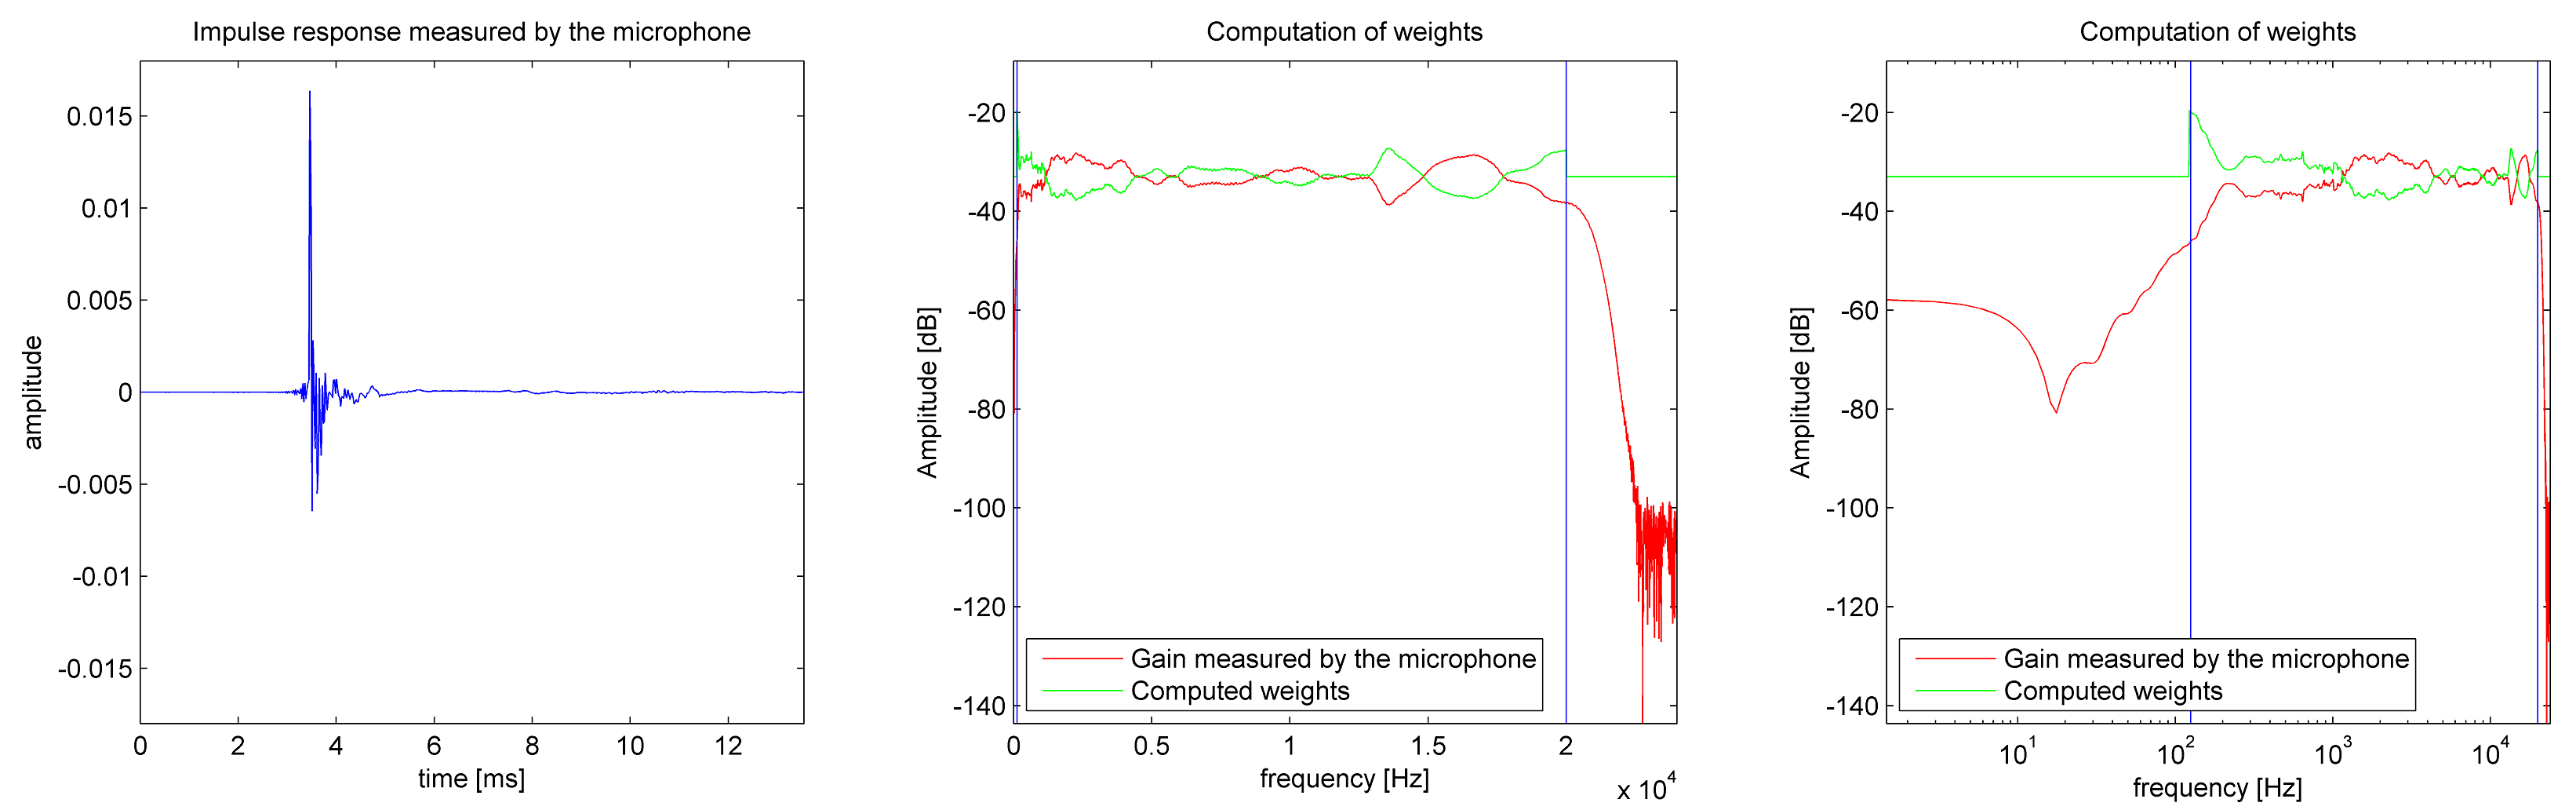
\includegraphics[width=\textwidth]{afbeeldingen/plots/weights.png}
    \caption[Computation of the weights]{Computation of the weights. The left plot contains the first 650 samples of the impulse response measured by the microphone.\\
    The two right plots both contain the same data, plotted linear and logarithmic. The computed weights are added to the mean value to show when the weights are added to the gain there will be a flat frequency response between $f_\text{min}$ and $f_\text{max}$ (given by the blue lines).}
    \label{fig:weights}
\end{figure}

Because these weights are for given frequencies, they need to be added per frequency.
Assume the signal $x_\text{phone}[n]$, first it will be transformed to the Fourier domain to $X_\text{phone}$.
In the signal $X_\text{phone}$ is information about the gain and the delay for a given frequency.
When the gain of this signal is computed, the weights per frequency are added and the gain plots can be made.

For further use in the beamformer however, the phase information is rather important.
If the gain of the signal is changed to decibel $(a_\text{dB}=20\log_{10}|a|\text{, with }a\in\mathbb{C})$ and transformed back $a_\text{mag}=\left(10^\frac{a_\text{db}}{20}\right)\text{, with }a_\text{mag}\in\mathbb{R})$ the result of the decibel to magnitude operation is a real (and positive) number, but the original signal was complex.
So, if we only apply the weights, as for the plots, the original phase information will be lost.
To keep the original phase information, the ratio between the magnitudes of the equalized and the original data will be computed and this ratio, $\alpha$ $(\in\mathbb{R}\backslash [-\infty,0\rangle)$, will be multiplied with the original signal, to retain phase information.\footnote{This can also be done by not taking the $\log$ of the signal and just use the ratio between the length of the signal before after applying the weights. The weights can be determined as ratios too.}
An example with $b\in\mathbb{C}$, with $j$ the imaginary unit can be found in equation \eqref{eq:b=bejp}

\begin{equation}
\label{eq:b=bejp}
\begin{split}
b&=|b|e^{j\arg(b)}\\
&=|b|e^{j\phi},\\
\alpha\cdot b&=\alpha \cdot |b|e^{j\phi}\\
&=|\alpha b|e^{j\phi}.
\end{split}
\end{equation}

The weights contain some 'noise'-like pattern on the overall line.
These are artefacts from the acoustic system and the microphone, which are not representable for the system.
To not let this influence the Log-equalizer, a low-pass filter is applied on the weights: $w*\frac{1}{7}\left[1~1~1~1~1~1~1\right]=w_\text{smooth}$.
The smoothened weights are thereafter used.
The removed noise pattern is shown with the blue line in Figure \ref{fig:weightsonmic} on page \pageref{fig:weightsonmic}, where one also sees the flattening working of the inverse filter on the gain measured by the microphone.

% figuur aan het einde van de paragraaf:
\begin{figure}[b!]
    \centering
    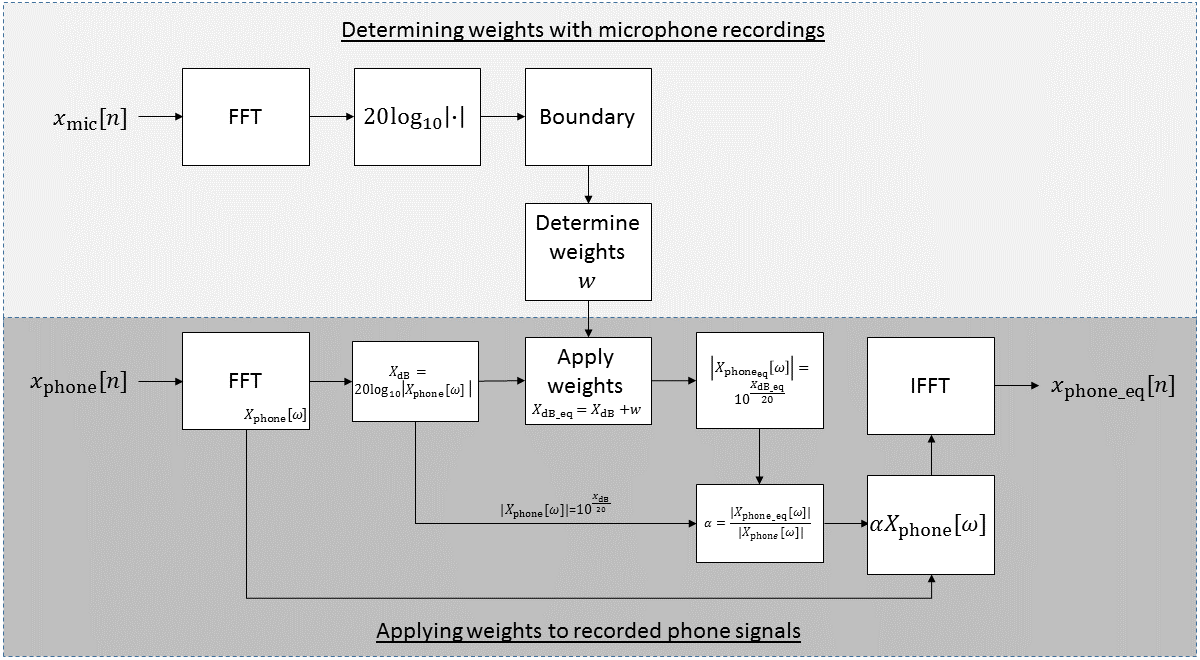
\includegraphics[width=\textwidth]{afbeeldingen/log_equalizer.png}
    \caption[Overview Log-equalizer]{Overview of the Log-equalizer, with preserved phase (based on \cite{Thomas2006})}
    \label{fig:Log-eq}
\end{figure}

\section{Results after equalization}
\label{sec:eq-prelim}
Applying the Log-equalizer to the phone recordings gives us the result in Figure \ref{fig:weightsonphone} on page \pageref{fig:weightsonphone}.
Applied on all phone recordings, the difference between the result after Chapter \ref{chap:measurements} and the equalized result is given in Figure \ref{fig:06-eq-lin}, on page \pageref{fig:06-eq-lin} (the settings stated in Section \ref{sec:eq-proc_rec} are also applied on the equalized figures).
In Figure \ref{fig:after-eq-log} the equalized data is displayed on a logarithmic frequency-axis so it is better comparable to the results of Gaubitch et al. \cite{Gaubitch2014} in Figure \ref{fig:Gaubitch} (page \pageref{fig:Gaubitch}).

The equalized gain is much better comparable to the results of Gaubitch et al. and therefore the Log-equalizer is used on all the smartphone recordings.
For different days of measurement, different microphone recording are available to determine the weights for the Log-equalizer.

\section*{Equalization - Conclusion}
After eliminating measurement errors caused by the difference in start time of playing and recording the sound signal, a reference point of no gain (0 dB) has been chosen (the equalized datapoint at $f=200\text{ Hz,}~\phi=90^\circ,~\theta=0^\circ)$.
The next part of this chapter consisted of the design of the equalizer, the solutions to solve the inverse filter if it is assumed \textit{linear} and time-invariant.
The assumption that the inverse filter is LTI is rejected and a Log-equalizer design is presented to equalize the data-sets from the measurements.

\clearpage
\invisiblesection{Figures}
\begin{figure}[t!]
        \centering
        \caption[Adding weights to microphone and smartphone microphone]{The result of adding the determined weights on two signals: the microphone and a smartphone measurement.}
        
        \label{fig:weightson}
        \begin{subfigure}[t]{\textwidth}
			    \caption{Equalizing the mean of the gain of 40 microphone measurements.}
			    \label{fig:weightsonmic}
                \centering
    			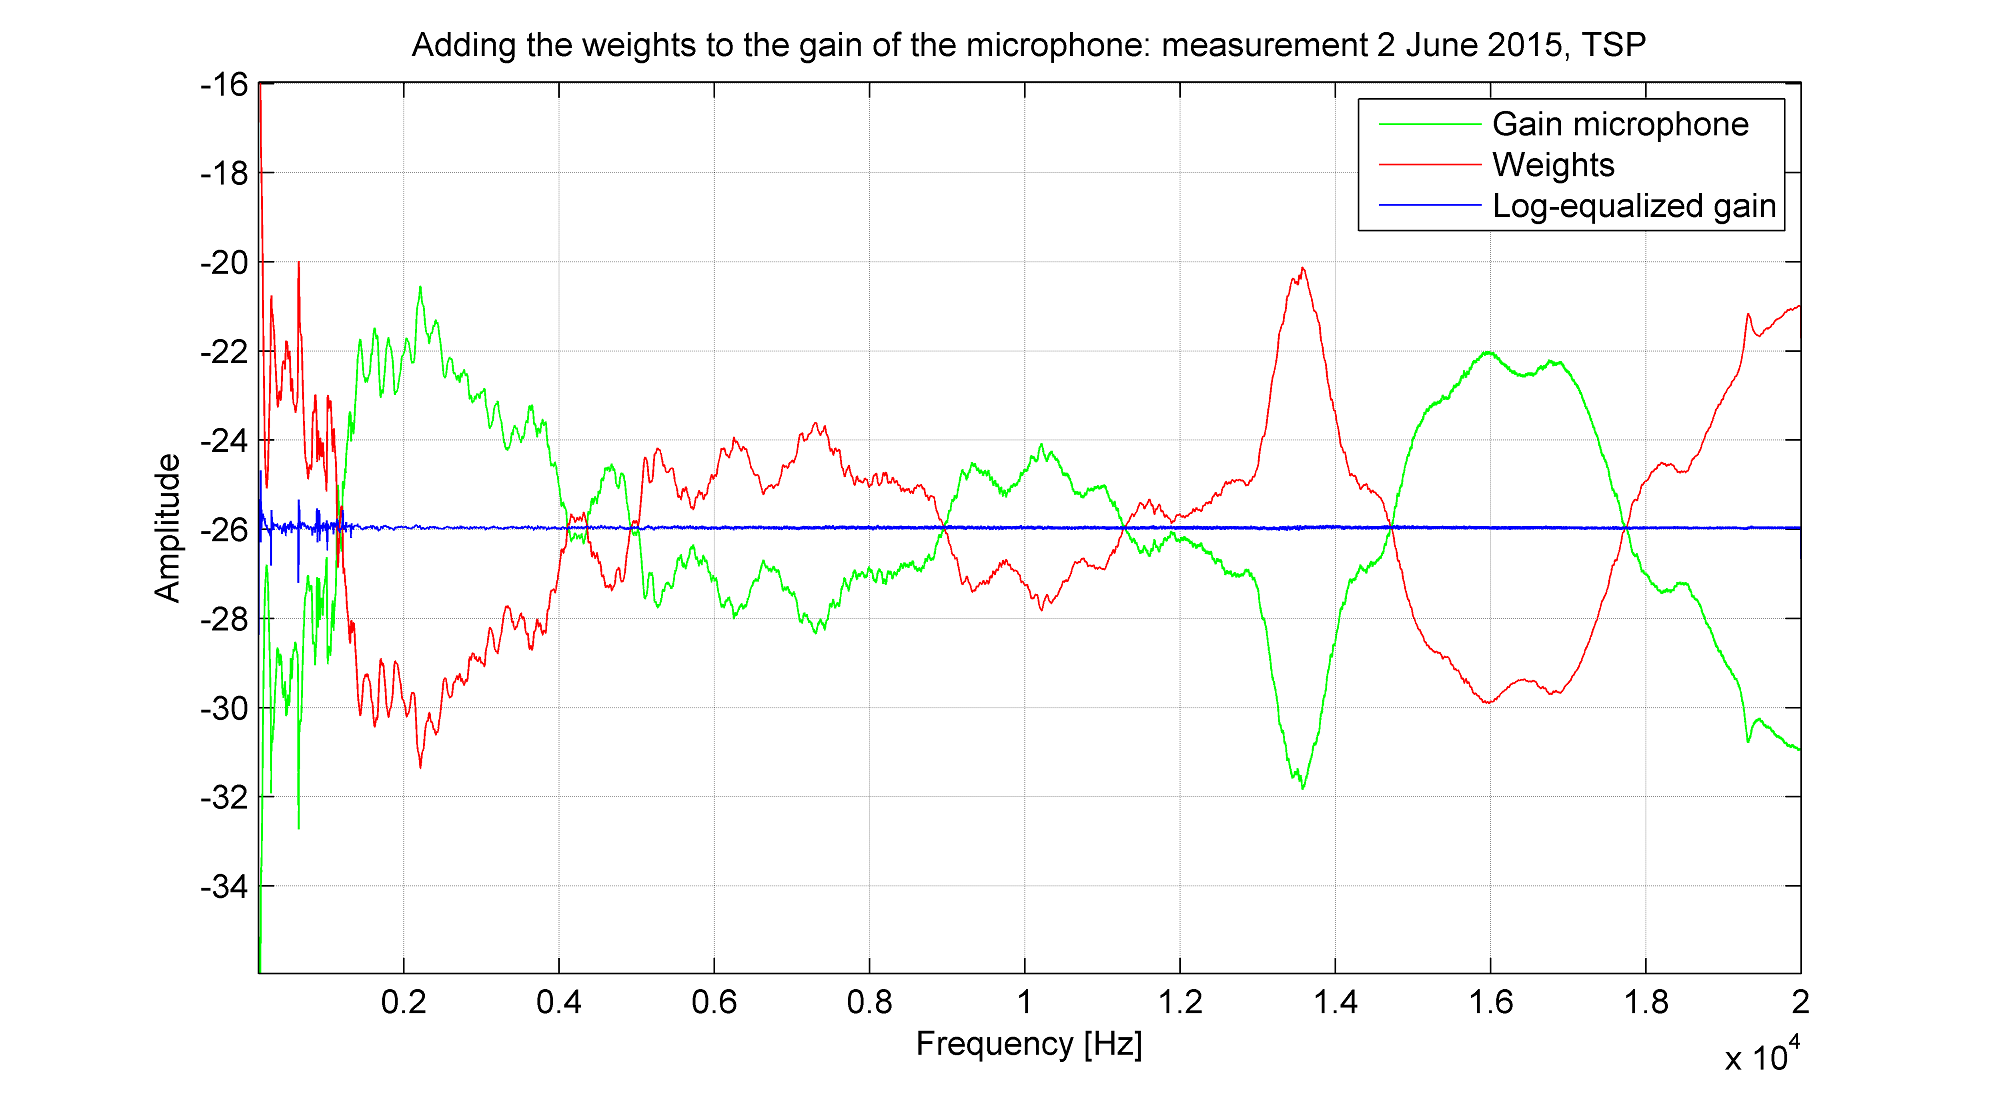
\includegraphics[width=\textwidth]{afbeeldingen/plots/weights-applied-microphone.png}
        \end{subfigure}%
        
        \begin{subfigure}[t]{\textwidth}
			    \caption{Equalizing the gain of {\nexus}, labelled with number 6, at $\phi=90^\circ$ and $\theta=0^\circ$}
			    \label{fig:weightsonphone}
                \centering
    			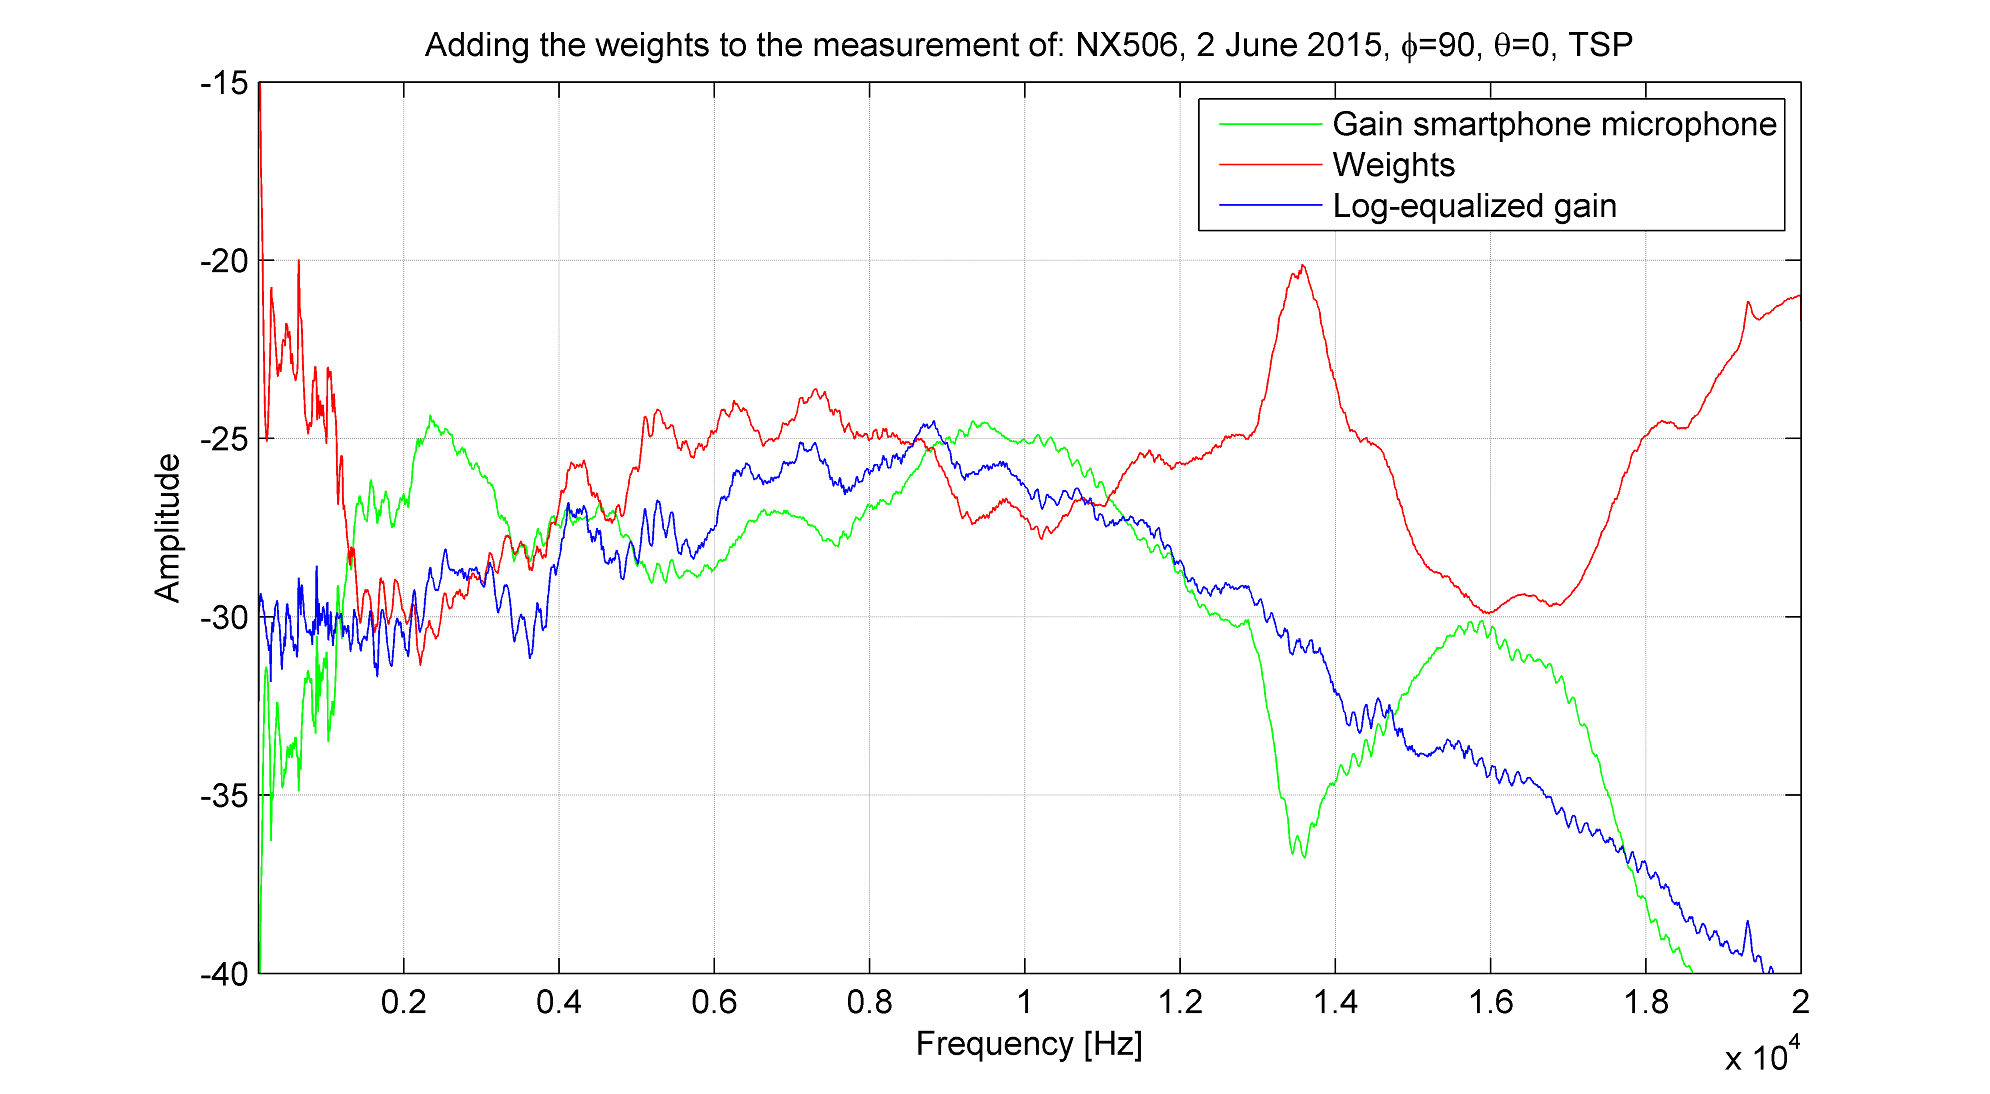
\includegraphics[width=\textwidth]{afbeeldingen/plots/weights-applied-smartphonemicrophone.png}
        \end{subfigure}
\end{figure}

\clearpage
\begin{figure}[t!]
        \centering
        \caption[Preliminary measurement results {\nexus} (6), equalized]{Preliminary measurement results of {\nexus}, labelled with number 6, at $\phi=90$ degrees, with limited frequency axis (from 125 Hz to 20 kHz) for the TSP measurement, non-equalized versus equalized.}
        \label{fig:06-eq-lin}
        \begin{subfigure}[t]{0.5\textwidth}
			    \caption{Non-equalized data on a linear frequency-scale}
			    \label{fig:before-eq-lin}
                \centering
    			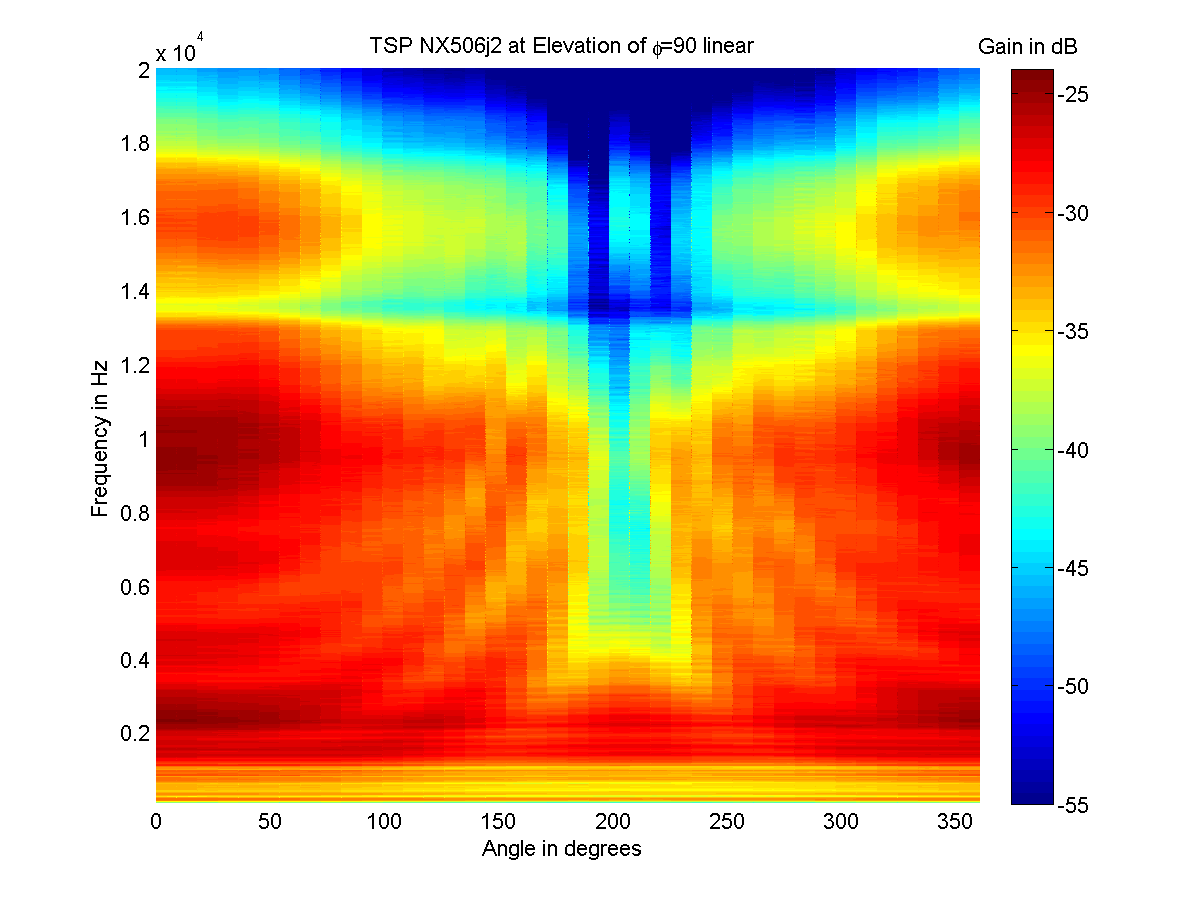
\includegraphics[width=\textwidth]{afbeeldingen/plots/NX506j2_TSP_090_lin.png}
        \end{subfigure}~
        \begin{subfigure}[t]{0.5\textwidth}
			    \caption{Equalized data on a linear frequency-scale}
			    \label{fig:after-eq-lin}
                \centering
    			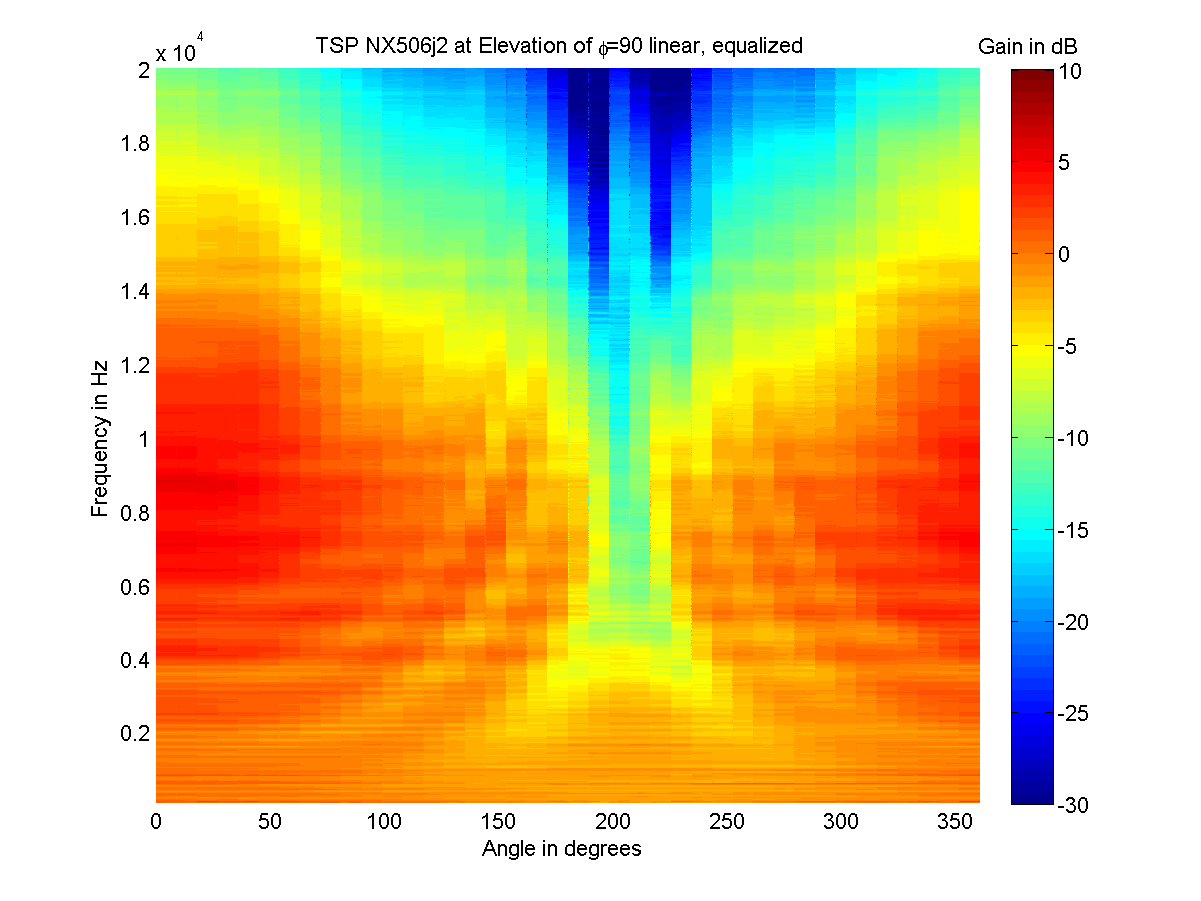
\includegraphics[width=\textwidth]{afbeeldingen/plots/NX506j2_TSP_090_lin_eq.png}
        \end{subfigure}
        
        \begin{subfigure}[t]{0.5\textwidth}
                \centering
			    \caption{Non-equalized data on a logarithmic frequency-scale}
			    \label{fig:before-eq-log}
    			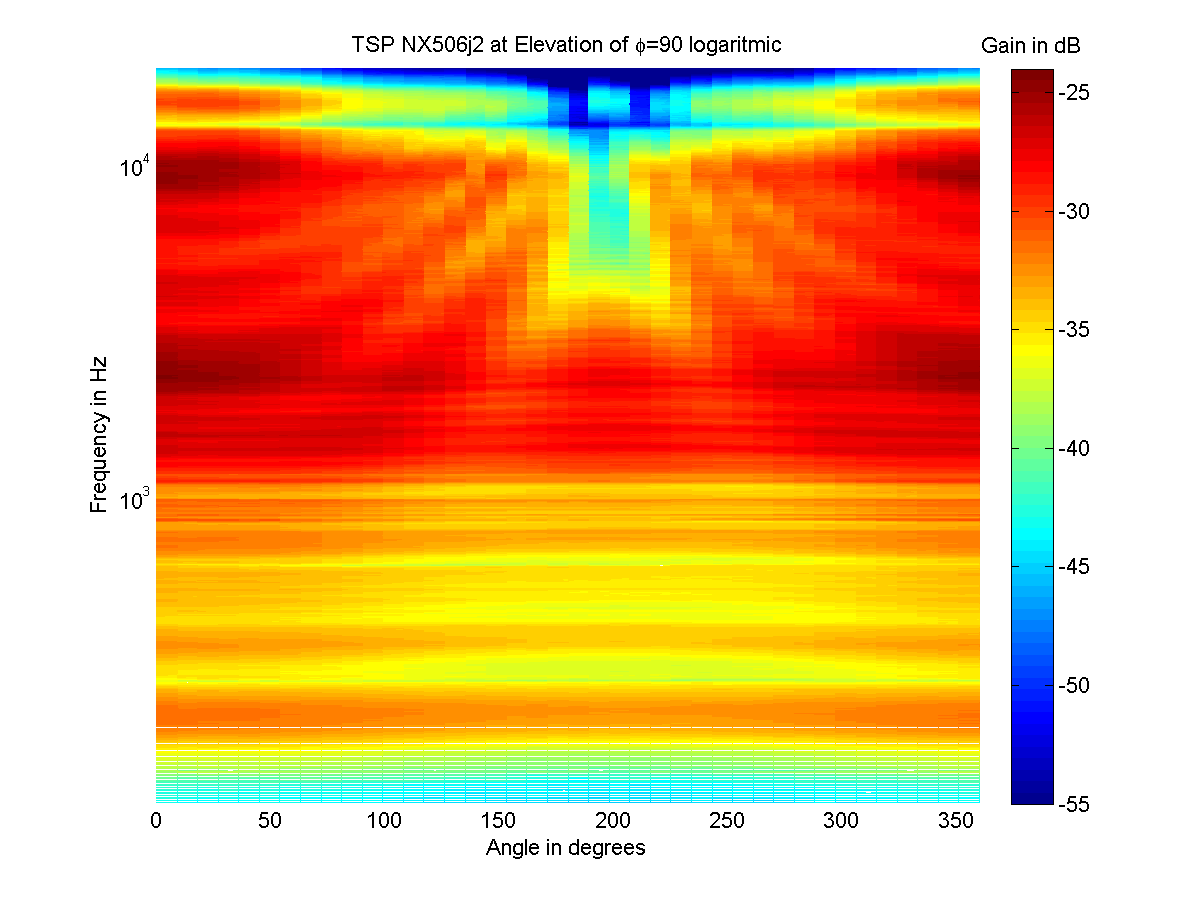
\includegraphics[width=\textwidth]{afbeeldingen/plots/NX506j2_TSP_090_log.png}
        \end{subfigure}~
        \begin{subfigure}[t]{0.5\textwidth}
                \centering
			    \caption{Equalized data on a logarithmic frequency-scale}
			    \label{fig:after-eq-log}
    			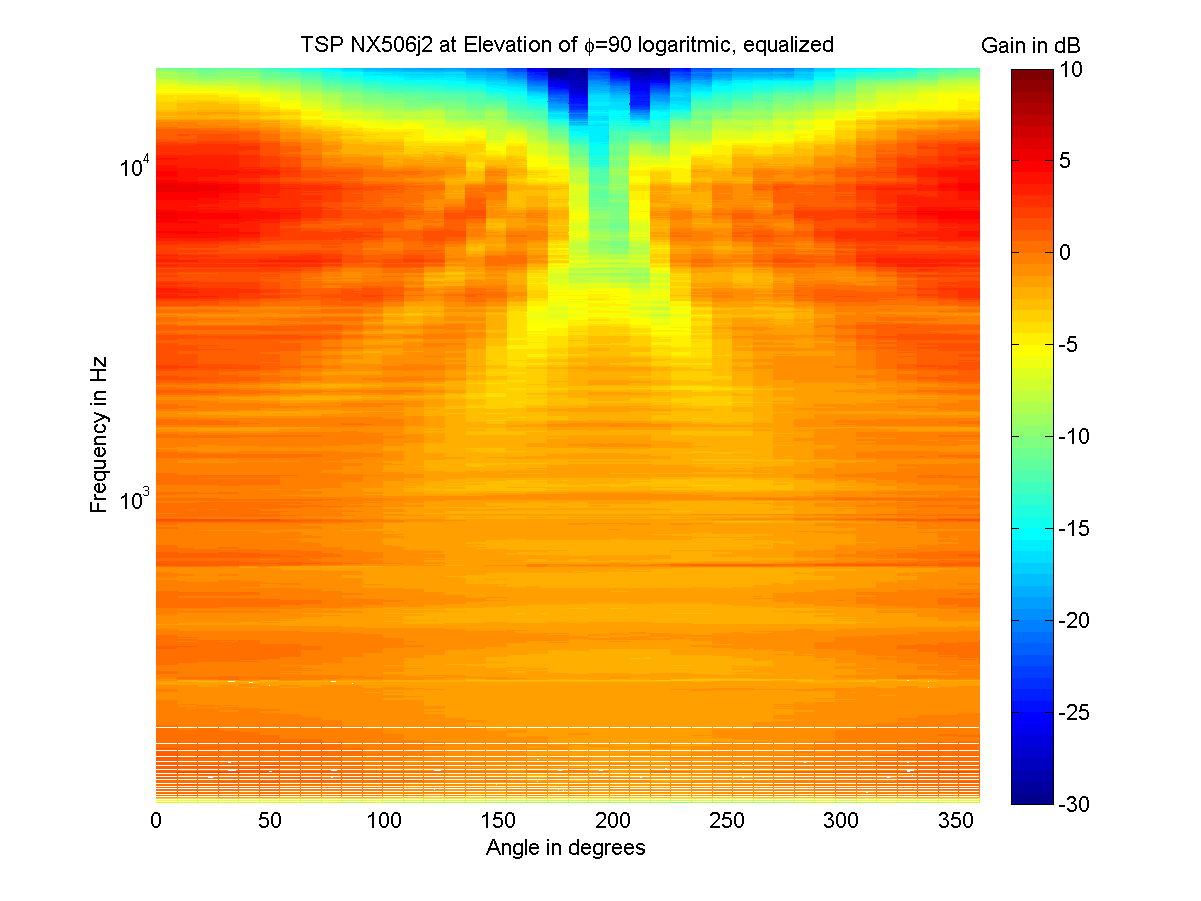
\includegraphics[width=\textwidth]{afbeeldingen/plots/NX506j2_TSP_090_log_eq.png}
        \end{subfigure}
\end{figure}